\section*{Aufgaben 2 und 3}
In dieser Aufgabe sollte die Latenzzeit und die Bandbreite gemessen werden, die
beim kommunizieren zwischen mehreren Prozessen auftreten. Dafür wurde mit verschiedenen
Konfigurationen von beteiligten Prozessoren und Zahlen von Prozessen die Zeit gemessen,
die benötigt wird, um eine Nachricht variabler Länge von einem Prozess zum anderen
und zurück zu senden. Dabei wurde dieser Ablauf $1000$ mal wiederholt und die 
gemessene Zeit gemittelt. Der Quelltext dafür ist in \lref{pingpong} und die darin
aufgerufene Funktion in \lref{walltime} dargestellt.

\lstinputlisting[label=lst:pingpong,caption={pingpong.c}]{../code/02/pingpong.c}
\lstinputlisting[label=lst:walltime,caption={wall\_time.c}]{../code/02/wall_time.c}

Wenn man für alle geforderten Konfigurationen die Zeiten in Abhängigkeit von der
Nachrichtenlänge aufträgt, resultiert der in \fref{zeiten} dargestellte Plot.

\begin{figure}[htb]
  \centering
  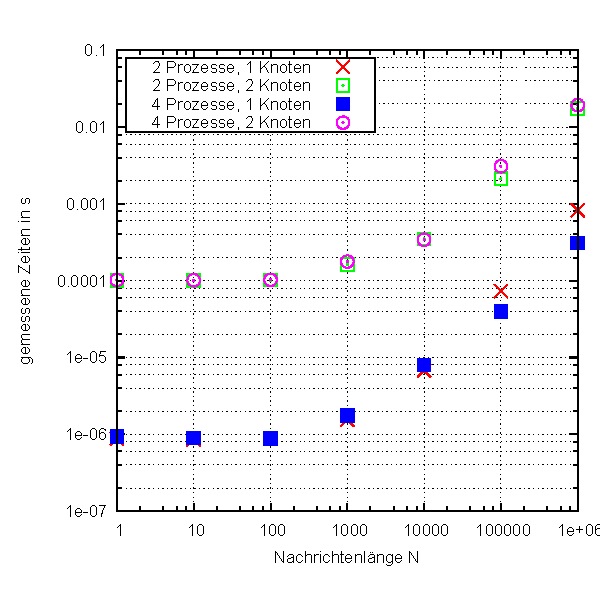
\includegraphics[width=0.8\columnwidth,keepaspectratio]{../tmp/zeiten}
  \caption{Gemessene Zeiten für das Senden einer Nachricht von einem Prozess zum
  anderen und zurück in Sekunden in Abhängigkeit von der Nachrichtenlänge}
  \label{fig:zeiten}
\end{figure}

Wie man erkennen kann, verläuft die Kommunikation zwischen mehreren Knoten generell
langsamer als die zwischen Prozessen, die auf dem gleichen Knoten laufen. Dies war 
zu erwarten, da die einzelnen Knoten über eine vergleichsweise langsame Netzwerkschnittstelle
miteinander verbunden sind, hingegen können die Prozesse auf einem Knoten mit Hilfe
eines internen Busses Informationen austauschen, der deutlich schneller Daten
transportieren kann als externe Verbindungen.

Weiterhin wird deutlich, dass die Nachrichtenlänge für die Arbeit mit mehreren
Knoten für kleine Längen (bis ca. $1000$ Zeichen) kaum einen Einfluss auf die
benötigten Zeiten hat. Demnach ist hier eindeutig die Wahl des Kommunikationsweges
das hemmende Element. Für größere Längen steigt die benötigte Zeit etwa nach einem 
Potenzgesetz (sogar annähernd linear) an. 

Auch die Zahl der Prozesse hat einen verschwindenden Einfluss, da vor allem bei der
Verwendung von nur einem Knoten die gemessenen Zeiten für zwei und vier Prozesse
übereinstimmen. Doch auch für zwei Knoten stimmen die Zeiten bis zu Nachrichtenlängen 
von etwa $10000$ überein, danach ist die Übertragung für vier Prozesse um einen Faktor
von etwa zwei langsamer als für zwei Prozesse. \textcolor{red}{wieder memory?}

Die Latenzzeit für die Kommunikation zwischen zwei Knoten lässt sich aus den entsprechenden
Kurven abschätzen. Für sehr kurze Längen spielt die zu übertragende Nachricht keine Rolle,
der dominierende Zeitfaktor kommt hier durch die Latenz ins Spiel. Diese liegt demnach bei
ca. $0.1$ Millisekunden für den Hin- und Rücktransport, also etwa bei $0.05$ Millisekunden
für jedes einzelne Senden einer Nachricht.

Auch wenn man nur auf einem Computer arbeitet, kann eine Latenzzeit gemessen werden.
Diese ist aber mit ca. $0.5$ Mikrosekunden etwa zwei Größenordnungen geringer als die
für die Kommunikation zwischen mehreren Knoten.

Die Bandbreite lässt sich aus dem Anstieg bestimmen, der bei großen Nachrichtenlängen
auftritt. Wenn man von den gemessenen Zeiten die Latenzzeit abzieht und dann die
übermittelte Datenmenge durch die übrig gebliebene Zeit dividiert, so erhält man 
die Bandbreite der Übertragung. Dies wurde für alle Nachrichtenlängen getan, woraus
der Plot in \fref{bandbreite} resultiert.

\begin{figure}[htb]
  \centering
  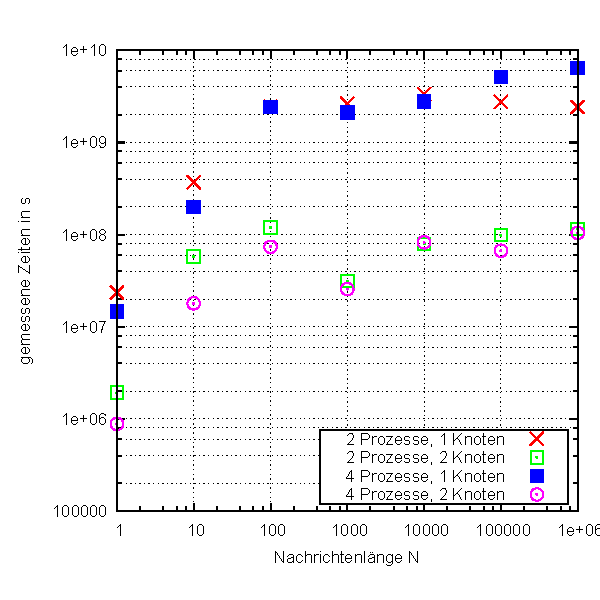
\includegraphics[width=0.8\columnwidth,keepaspectratio]{../tmp/bandbreite}
  \caption{Gemessene Bandbreite für das Senden einer Nachricht von einem Prozess zum
  anderen in MByte pro Sekunde in Abhängigkeit von der Nachrichtenlänge}
  \label{fig:bandbreite}
\end{figure}

Die Bandbreite für die Kommunikation zwischen mehreren Knoten liegt also bei etwa 
100 MByte pro Sekunde, was in etwa der möglichen Geschwindigkeit in einem LAN entspricht (eine
übliche Größe ist  ein GBit pro Sekunde). Für die Kommunikation innerhalb eines Knoten 
erreicht die Bandbreite Werte von ca. acht Gigabyte pro Sekunde. Auch dies ist ein
realistischer Wert für die Kommunikation zwischen Komponenten innerhalb eines Computers.

Für alle Messungen muss beachtet werden, dass die Ergebnisse von der aktuellen Auslastung
der verwendeten Knoten abhängen können und somit nur als Näherung gelten können. Für 
unsere Messungen haben wir Knoten gewählt, auf denen keine weiteren Nutzer angemeldet waren.